% THIS IS SIGPROC-SP.TEX - VERSION 3.1
% WORKS WITH V3.2SP OF ACM_PROC_ARTICLE-SP.CLS
% APRIL 2009
%
% It is an example file showing how to use the 'acm_proc_article-sp.cls' V3.2SP
% LaTeX2e document class file for Conference Proceedings submissions.
% ----------------------------------------------------------------------------------------------------------------
% This .tex file (and associated .cls V3.2SP) *DOES NOT* produce:
%       1) The Permission Statement
%       2) The Conference (location) Info information
%       3) The Copyright Line with ACM data
%       4) Page numbering
% ---------------------------------------------------------------------------------------------------------------
% It is an example which *does* use the .bib file (from which the .bbl file
% is produced).
% REMEMBER HOWEVER: After having produced the .bbl file,
% and prior to final submission,
% you need to 'insert'  your .bbl file into your source .tex file so as to provide
% ONE 'self-contained' source file.
%
% Questions regarding SIGS should be sent to
% Adrienne Griscti ---> griscti@acm.org
%
% Questions/suggestions regarding the guidelines, .tex and .cls files, etc. to
% Gerald Murray ---> murray@hq.acm.org
%
% For tracking purposes - this is V3.1SP - APRIL 2009

\documentclass{acm_proc_article-sp}
\usepackage{algorithm}
\usepackage{algorithmicx}
\usepackage[noend]{algpseudocode}
\algrenewcomment[1]{\(\triangleright\) #1}
\usepackage{hyperref}


\begin{document}

\title{Data Fusion Using Source Trustworthiness}
%
% You need the command \numberofauthors to handle the 'placement
% and alignment' of the authors beneath the title.
%
% For aesthetic reasons, we recommend 'three authors at a time'
% i.e. three 'name/affiliation blocks' be placed beneath the title.
%
% NOTE: You are NOT restricted in how many 'rows' of
% "name/affiliations" may appear. We just ask that you restrict
% the number of 'columns' to three.
%
% Because of the available 'opening page real-estate'
% we ask you to refrain from putting more than six authors
% (two rows with three columns) beneath the article title.
% More than six makes the first-page appear very cluttered indeed.
%
% Use the \alignauthor commands to handle the names
% and affiliations for an 'aesthetic maximum' of six authors.
% Add names, affiliations, addresses for
% the seventh etc. author(s) as the argument for the
% \additionalauthors command.
% These 'additional authors' will be output/set for you
% without further effort on your part as the last section in
% the body of your article BEFORE References or any Appendices.

\numberofauthors{3} %  in this sample file, there are a *total*
% of EIGHT authors. SIX appear on the 'first-page' (for formatting
% reasons) and the remaining two appear in the \additionalauthors section.
%
\author{
% You can go ahead and credit any number of authors here,
% e.g. one 'row of three' or two rows (consisting of one row of three
% and a second row of one, two or three).
%
% The command \alignauthor (no curly braces needed) should
% precede each author name, affiliation/snail-mail address and
% e-mail address. Additionally, tag each line of
% affiliation/address with \affaddr, and tag the
% e-mail address with \email.
%
% 1st. author
\alignauthor
Manual Heinkel \\
       \affaddr{UMass Amherst}\\
       \affaddr{140 Governors Drive}\\
       \affaddr{Amherst, Massachusetts}\\
       \email{heinkel@cs.umass.edu}
% 2nd. author
\alignauthor
Nicholas Monath \\
       \affaddr{UMass Amherst}\\
       \affaddr{140 Governors Drive}\\
       \affaddr{Amherst, Massachusetts}\\
       \email{nmonath@cs.umass.edu}
% 3rd. author
\alignauthor 
Lakshmi Nair \\
       \affaddr{UMass Amherst}\\
       \affaddr{140 Governors Drive}\\
       \affaddr{Amherst, Massachusetts}\\
       \email{lvnair@cs.umass.edu}
}
\date{8 March 2015}
% Just remember to make sure that the TOTAL number of authors
% is the number that will appear on the first page PLUS the
% number that will appear in the \additionalauthors section.

\maketitle


% A category with the (minimum) three required fields
%\category{H.4}{Information Systems Applications}{Miscellaneous}
%A category including the fourth, optional field follows...
%\category{D.2.8}{Software Engineering}{Metrics}[complexity measures, performance measures]

%\terms{Theory}

%\keywords{ACM proceedings, \LaTeX, text tagging} % NOT required for Proceedings

\section{Introduction}

The advent of data sources on the web in the last two decades has sparked the need for automated methods of combining sources into a single source. As these data sources often contain noisy and incorrect data, techniques for discerning the correct value among a set of conflicting values must be developed. These techniques solve the problem of data fusion. In data fusion, we consider information or $attributes$ of $entities$ provided by various $sources$. The entities include companies, airplane flights, books etc and attributes for these entities include open and close prices, time delays and isbn numbers respectively. Data sources include any site or database on the web. Data fusion is challenging in that the data may be stored in a variety of formats. Values for an entity's attributes may be semantically equivalent without having the same representation (e.g \$104Mil and 104,000,000 as a company's holding or Ernest Hemingway and E. Hemingway as the author of a book). In certain cases, the range of values for an attribute is not known. The decision of selecting the correct value for an attribute must be made under a great deal of uncertainty in a situation that is heavily domain dependent. Typically, no prior knowledge is known about the authenticity of the data sources. Labeled data is scarce and so supervised methods for data fusion are not practical. Most approaches to data fusion are unsupervised and make use of algorithms such as Expectation-Maximization (EM). A further difficulty is that the causes of erroneous data cannot easily be modeled by common distributions. Many of the current approaches to data fusion in the literature currently focus on modeling the trustworthiness of a data source. However, it is possible that a data source reliably provides values for one attribute, but not others. For example, Orbitz might accurately provide the departure time of a flight while frequently providing an incorrect value for the delay of a flight. In this work, we present models of the trustworthiness each attribute provided by a source. Attributes of entities are often assumed to be independent. We propose a possible model which captures the trustworthiness of sources as well as dependence among attributes.  Other methods in the literature model copying between data sources and the variance of the attributes. Few approaches consider all of these well studied features. We hope to investigate if we can come up with a model which covers all of these features. 

\section{Related Work}
Data fusion is also referred to as truth discovery \cite{waguih:truth} \cite{yin:truth} and data integration \cite{sarma:data} \cite{zhao:bayesian}. While there has been some work on how data fusion pertains to information extraction, specifically question answering \cite{wu:corroborating}, the significant body of literature pertains to the construction of databases, particularly relational databases and, recently, knowledge bases \cite{dong:data}. 



The problem of data fusion in relational databases typically consists of multiple phases \cite{bleiholder:data} \cite{li:truth}. Given a collection of data sources, which all contain data that is to be stored in a particular relation, the first step is often the mapping of the data sources' schema to the schema of the underlying relation \cite{bleiholder:data}. Several techniques for schema mapping are discussed in \cite{naumann:data}. Several papers such as \cite{li:truth} address the process of selecting the true data values from the sources independently of schema mapping as we do in this work.


A naive approach to this problem is to resolve the conflicts by performing a majority vote among the sources. Early approaches such as {\sc TruthFinder} \cite{yin:truth} extend this technique by incorporating a notion of source trustworthiness, i.e. how much one should trust the value presented by a source. {\sc TruthFinder} follows a heuristic which assumes that a source which provides mostly true claims for many data items is likely to provide true claims for other data items. The estimation of the trustworthiness of data sources   is a common thread among data fusion algorithms as noted by \cite{li:truth} \cite{waguih:truth}. Other truth discovery algorithms which are based on corroboration have been proposed by Galland et al. \cite{galland:corro}. Three algorithms were proposed ({\sc Cosine}, {\sc 2-Estimates} and {\sc 3-Estimates}) which estimate the truth in the values and the trust in the views. {\sc Cosine} is a heuristic approach which is based on the cosine similarity in information retrieval. The algorithm is initialized with the confidence of each value and the source trustworthiness. The algorithm then iteratively recomputes the source trustworthiness as a linear function of the previous iteration. 


Other approaches such as Latent Truth Model proposed by Zhao et al. \cite{zhao:bayesian} use probabilistic Bayesian models. In contrast to previous methods, this model captures the distinction between false positive and false negative errors injected by the source. LTM models the probability of each fact being true as a latent random variable and the actual truth label of each fact as a latent boolean random variable. A Collapsed Gibbs Sampling algorithm is used for inferring the true labels. The algorithm works by randomly initializing the truth labels for each fact and in each iteration the truth values are sampled from a distribution conditioned on all current truth labels. 

Another method proposed by Wang et al. \cite{wang2012truth} is Maximum Likelihood Estimation. Unlike most of the other methods, which are heuristic, this approach offers an optimal solution to the problem of truth discovery. The model parameters include the probability of a value being reported as true by the source and the probability that value is true given the source. The Expectation Maximization Algorithm is used to find optimal values for these parameters. During the Expectation step, the probability that value is true given source probabilities is computed and during the Maximization step, the source probabilities are computed. This method has been shown to work well in cases where there is a lot of noise in the input data. 

Related algorithms such as Latent Credibility Analysis (LCA) \cite{pasternack:latent} model the truthfulness of facts presented by sources using a probabilistic graphical model. LCA represents the truth of a given fact as a latent variable in the graphical model. LCA jointly models the truth of a given fact, the trustworthiness of all of the data sources and other factors such as the variability of particular attributes. Unlike many other works, LCA can be trained not only in an unsupervised way, but also in a semi-supervised way. LCA follows up earlier work done by the same authors such as \cite{pasternack:knowing} and \cite{pasternack:making}, which uses an interesting trick of placing sources into several groups in the truth finding process. 


Data sources may also contain noise as a result of copying values from one another. A novel contribution of \cite{dong:integrating} is a model of the dependence between sources. The {\sc AccuCopy} method presented in \cite{dong:integrating} and in the survey \cite{li:truth} models the dependence by estimating the probability a source would independently come up with its claim using a Bayesian approach. 

The problem of data fusion is extended to data streams in the recent work \cite{zhao:truth}. The probabilistic approach performs fusion via source quality estimation in real time. While the approach could be used on fixed data as well, the efficiency of this approach is an important contribution. 

The recent work of Li et al. \cite{li:resolving} has been shown to be state of the art on several standard datasets such as the stock dataset \cite{li:truth}, the flight dataset \cite{li:truth} and others. The work frames data fusion as a regularized optimization problem such that the loss function cleverly combines a representation of source trustworthiness and the values proposed by each source while respecting the domain of the attributes. As in LCA and other methods, the trustworthiness is calculated jointly. As one of the top performing systems, this work will be a point of comparison and extension in our project. 

Recent work has focused on knowledge fusion, a closely related problem to data fusion \cite{dong:data} \cite{pochampally:fusing} \cite{yu:wisdom}.  In this task the data are knowledge base entries such as a pair of entities and a relation rather than a collection of attributes. Many data fusion techniques can be effectively applied to this problem as shown in \cite{dong:data}. Handling data sources which contain correlations is addressed by \cite{pochampally:fusing}. Correlations between sources include not only copying, but also factors such as similarities between the extraction techniques used. Modeling correlations rather than copied values is a novel contribution by  \cite{pochampally:fusing}.


Another related research area is the collection of labels from crowdsourcing \cite{nguyen:minimizing}. Particularly, techniques for using crowdsourcing to create labeled data sets \cite{sheng:get} \cite{nguyen:minimizing} and crowdsourcing for multiple choice question answering \cite{bachrach:grade}. In these approaches the number of sources/users can be much greater than for usual data fusion problems \cite{li:truth} \cite{nguyen:minimizing}.

We expect our work to differ from the previous work in that we will model source trustworthiness not only globally, i.e. for all attributes, but also locally for each attribute. In doing so, we hope to capture a more fine grained representation of source trustworthiness. We will also attempt to ensemble existing algorithms using a variety of techniques such as weighted ensemble. We hope to use semi-supervised techniques in situations where more domain-knowledge could be useful. Most of the models presented previous works such as \cite{pasternack:latent} and \cite{li:resolving} do not attempt to measure the dependence of attributes on other attributes. We hope to investigate if there is a tractable way to capture these dependencies and if we can use them to improve data fusion methods.

\vspace{2cm}

\section{Models}

\subsection{Problem Description}

We provide the following formalism for the problem of data fusion. A $record$, $r$, is provided by a $source$, $s$, about an $entity$, $e$. A $source$ is a supplier of data. For example, Expedia is a source for flight data, and Yahoo Finance is a source of stock data.  An $entity$ is a real world object about which a $source$ provides data. The entities about which Expedia provides data are flights and Yahoo Finance provides data about a company's stock price. An entity has a unique identifier. In the case of flight data this would be the flight number. In the case of stock data, this would be the company's ticker symbol. A $record$ contains one or more $attributes$, $a_1,\ a_2,\dots,\ a_n$, of an entity. Each $attribute$ has a specific domain. In the case of flights, the attribute $time$ $delay$ might be an integer and for stocks, the $opening$ $price$ might have a domain of positive real numbers.  The domain of an attribute may also be binary (true/false) or categorical. We refer to the collection of records provided by a source $s$ as $R_s$. The $schema$ of a record is the set of attributes which each entity is expected to contain.

Given a set of sources $S$ and a collection of records $R_s$ for each $s \in S$, the problem of \emph{data fusio}n is to combine all collections $R_s$ into a single collection $\hat{R}$ which estimates the true assignment of values to the attributes for entities in $R^*$.  Each of the following algorithms provides a different technique for converting a set of $R_s$ collections into $\hat{R}$. 

\subsection{Data Set}
To evaluate our algorithms we consider the \emph{stock data set}\footnote{\url{http://lunadong.com/fusionDataSets.html}} which was introduced in \cite{li:truth}. Some statistics of the data set is shown in table \ref{fig:stock}. This data set contains stock information obtained in July 2011 by using 55 different sources like \emph{Google Finance, Bloomberg} or \emph{NASDAQ}. From each of these sources 1000 stocks were considered. In July 2011 on each weekday the stock data of each stock was collected from each of the 55 sources. Different sources had different numbers of attributes (from 3 to 71). The \emph{clean stock data set} which we use contains 16 attributes per stock which had the best coverage across the sources. Among these 16 attributes are: \emph{change in \%, opening price, todays high/low, market capacity, dividend, etc}. For the stock \emph{stock data}, \emph{Xian Li et al.} \cite{li:truth} also generated a gold standard for evaluation.


%todo: change vertical padding
\begin{figure}[h]
    \centering
{%\footnotesize
\begin{tabular}{  | c | c | c | c  | c | c |}		
\hline
 \textbf{Src} & \textbf{Period} & \textbf{Stocks} & \textbf{Attributes}  & \textbf{Items}  \\
\hline
 55 & July 2011 &  1000 & 16 &  16000*55   \\
\hline
\end{tabular}
}
 \caption{Stock data collection overview}%
    \label{fig:stock}%
\end{figure}

\subsection{Implemented Existing Methods}

In this section, we present a more detailed explanation of the methods we have implemented so far. 

\subsubsection{Majority Voting}

A simple approach to data fusion is collect all of the candidate values provided by the sources for a particular attribute of an entity and assign the attribute the value that appears most frequently. While general idea appears in all of the following   algorithms,  it is flawed in that it ignores information about the data sources, uncertainty of the attributes and the relationships between  attributes.

\subsubsection{Cosine}

\subsubsection{2-Estimate}
The {\sc 2- Estimate} algorihtm was proposed by \emph{Galland et al.} in \cite{galland:corro}. This algorithm is related to a prababilistic model to estimate the source trustworthiness and the confidence of an attibute value. To compute the value confidence the algorithm takes the disagreeing sources into consideration. First, the confidence of a value is computed by analyzing agreeing and disagreeing sources of that value. After that the value confidence ins nomralized with a \emph{normalization function}. Then the algorithm recomputes the source trustworthiness by looking at the confidence of the different values provided by that source. After normalizing the source trustworthiness this process is repeated until convergence.


%% Lakshmi & Manuel please feel free to change these variable names if you want to. I'm in no way attached to them, it was just an initial stab at this. 
\begin{table}
\centering
\begin{tabular}{|c|c|}
\hline
Variable & Description  \\
\hline
$s$ & Data source \\
$S$ & Set of all sources  \\
$e$ & Entity \\
$E$ & Set of all entities \\
$a_i$ & The $i^{th}$ Attribute of $e$ \\
$\alpha_i^{(s)}$ & The value of $a_i$ given by $s$ \\
$Attr(e)$ & The attributes of $e$ \\
\hline
\end{tabular}
\caption{Definition of each variable used in the algorithms.}
\end{table}

\begin{table}
\centering
\begin{tabular}{|c|c|}
\hline
Variable & Example \\
\hline
$s$  & MarketWatch \\
$S$ & \{MarketWatch,YahooFinance,$\dots$\}  \\
$e$ & GM (General Motors) \\
$E$ & \{GM, AAPL, F, $\dots$\} \\
$a_i$ & Opening Price \\
$\alpha_i^{(s)}$ & \$37.50 \\
$Attr(e)$ & \{Open Price, Avg Price, $\dots$\} \\
\hline
\end{tabular}
\caption{Examples for each of the variable types.}
\end{table}

\subsubsection{TruthFinder}

Yin et al present a Bayesian approach to data fusion in \cite{yin:truth}.  The likelihood of an entity's attribute having a particular value is a function of both the trustworthiness of the source providing the value as well as the values presented by other sources. The model is based on the idea that a source is trustworthy if it frequently provides a correct value and a value is often correct for an attribute if the providing source is trustworthy. However, as the algorithm is unsupervised we model the trustworthiness of a source as a function of the likelihood of correctness of the attributes it provides. 

Specifically, let $\alpha_i^{(s)}$ be the value provided by source $s$ for the attribute $a_i$ of entity $e$. The $trustworthiness$ of $s$ is denoted: $\mathsf{TRUST}(s)$. Based solely on the trustworthiness of the sources, the likelihood of correctness or confidence we have that $\alpha_i^{(s)}$ is the correct value for $a_i$ is denoted $\mathsf{CONF(\alpha_i^{(s)})}$.  The confidence is defined (in log space) as:

\begin{equation}
\mathsf{CONF(\alpha_i^{(s)})} = \sum_{s' \in S} \mathsf{Provides}(s',\alpha_i^{(s)}) \cdot \ln(1-\mathsf{TRUST}(s'))
\end{equation}

where $\mathsf{Provides}(s',\alpha_i^{(s)})$ is an indicator function that is 1 only if $s'$ provides $\alpha_i^{(s)}$ as the value for $a_i$ and 0 otherwise. $\mathsf{CONF(\alpha_i^{(s)})}$ is the log probability that each of the sources providing the value $\alpha_i^{(s)}$ are correct. This confidence value is then used to create an $adjusted$ confidence $\mathsf{CONF^\star(\alpha_i^{(s)})}$.

\begin{align}
\mathsf{CONF^\star(\alpha_i^{(s)})} &= \mathsf{CONF(\alpha_i^{(s)})} + \\ \nonumber
&  \sum_{s' \in S \setminus \{s\}} \rho \cdot \mathsf{CONF(\alpha_i^{(s')})}  \cdot \mathsf{SIM}(\alpha_i^{(s)},\alpha_i^{(s')})
\end{align}

where $\mathsf{SIM}$ is a similarity function defined unique for domain the attribute $a_i$. The function $\mathsf{CONF}^\star$ can be view as increasing  the $\mathsf{CONF}$ of the value of an attribute if trustworthy sources provide similar values and decreasing it otherwise. As mentioned before the trustworthiness of a source based on the confidence values for the attributes it provides. 

\begin{equation}
\mathsf{TRUST}(s) = \frac{1}{Z} \sum_{e \in E}\sum_{a \in Attr(e)} \sigma(\gamma \cdot \mathsf{CONF}(\alpha^{(s)}))
\end{equation}

where $Z$ is the number of values (across all entities) provided by $S$ and $\sigma$ is the sigmoid function, which is used to map $\mathsf{CONF}^\star$ to a value between 0 and 1.

\begin{equation}
\sigma(x) = \frac{1}{1 + \exp{(-x)}}
\end{equation}


\subsection{Proposed Methods}

We are in the process of developing extensions to these techniques. Our extensions fall into three main categories: ensemble methods; source-attribute pairwise trustworthiness, and attribute dependence. Based on our literature survey, we do not believe that these topics have been thoroughly investigated thus far. 


\subsubsection{Ensemble Methods}

Ensembling existing techniques will consider a group of algorithms $\mathcal{A}_1,\mathcal{A}_2,\dots,\mathcal{A}_N$. Each algorithm $\mathcal{A}_i$ takes the as input an $R_s$ for each source $s \in S$ and outputs a collection of records $\hat{R}_{\mathcal{A}_i}$. 

Our first attempt at an ensemble method is to apply the majority voting algorithm on the outputs $\hat{R}_{\mathcal{A}_1}$, $\hat{R}_{\mathcal{A}_2}$, $\dots$,$\hat{R}_{\mathcal{A}_N}$. In this case, each of the algorithms acts a source. We will follow substitute majority voting with the other algorithms. In this way, we have a nested structure in which we learn a \emph{trustworthiness} of each algorithm. This approach is often referred to as \emph{stacking} in the literature. 

\subsubsection{Source Attribute Trustworthiness}

As pointed out in \cite{dong:truth}, a data source may reliably provide values for a particular attribute of an entity, but may unreliably provide values for another attribute. In response to this, we give extensions of existing algorithms which model the trustworthiness of a source--attribute pair.  The {\sc TruthFinder} algorithm can be extended by redefining the $\mathsf{CONF}$ and $\mathsf{TRUST}$ functions in the following way: 


\begin{equation}
\mathsf{CONF(\alpha_i^{(s)})} = \sum_{s' \in S} \mathsf{Provides}(s',\alpha_i^{(s)}) \cdot \ln(1-\mathsf{TRUST}(s',a_i))
\end{equation}


\begin{equation}
\mathsf{TRUST}(s,a_i) = \frac{1}{|E|} \sum_{e \in E} \sigma(\gamma \cdot \mathsf{CONF}(\alpha_i^{(s)}))
\end{equation}

where, with a slightly abuse of notation, $\alpha_i^{(s)}$ refers to the value supplied for attribute $a_i$ for each $e$ in the summation. The  $\mathsf{TRUST}$ is now parameterized at the attribute level; the trustworthiness of an attribute from a source is the average of the confidence values for those given attributes. The rest of the {\sc TruthFinder} algorithm remains unchanged. 


\begin{figure}
\centering
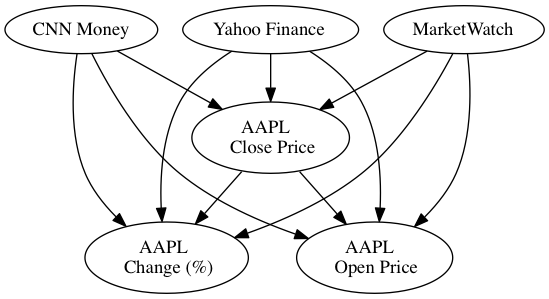
\includegraphics[width=5cm]{bn1.png}
\caption{An example of the attribute dependence model, which models source trustworthiness.}
\end{figure}

\begin{figure}
\centering
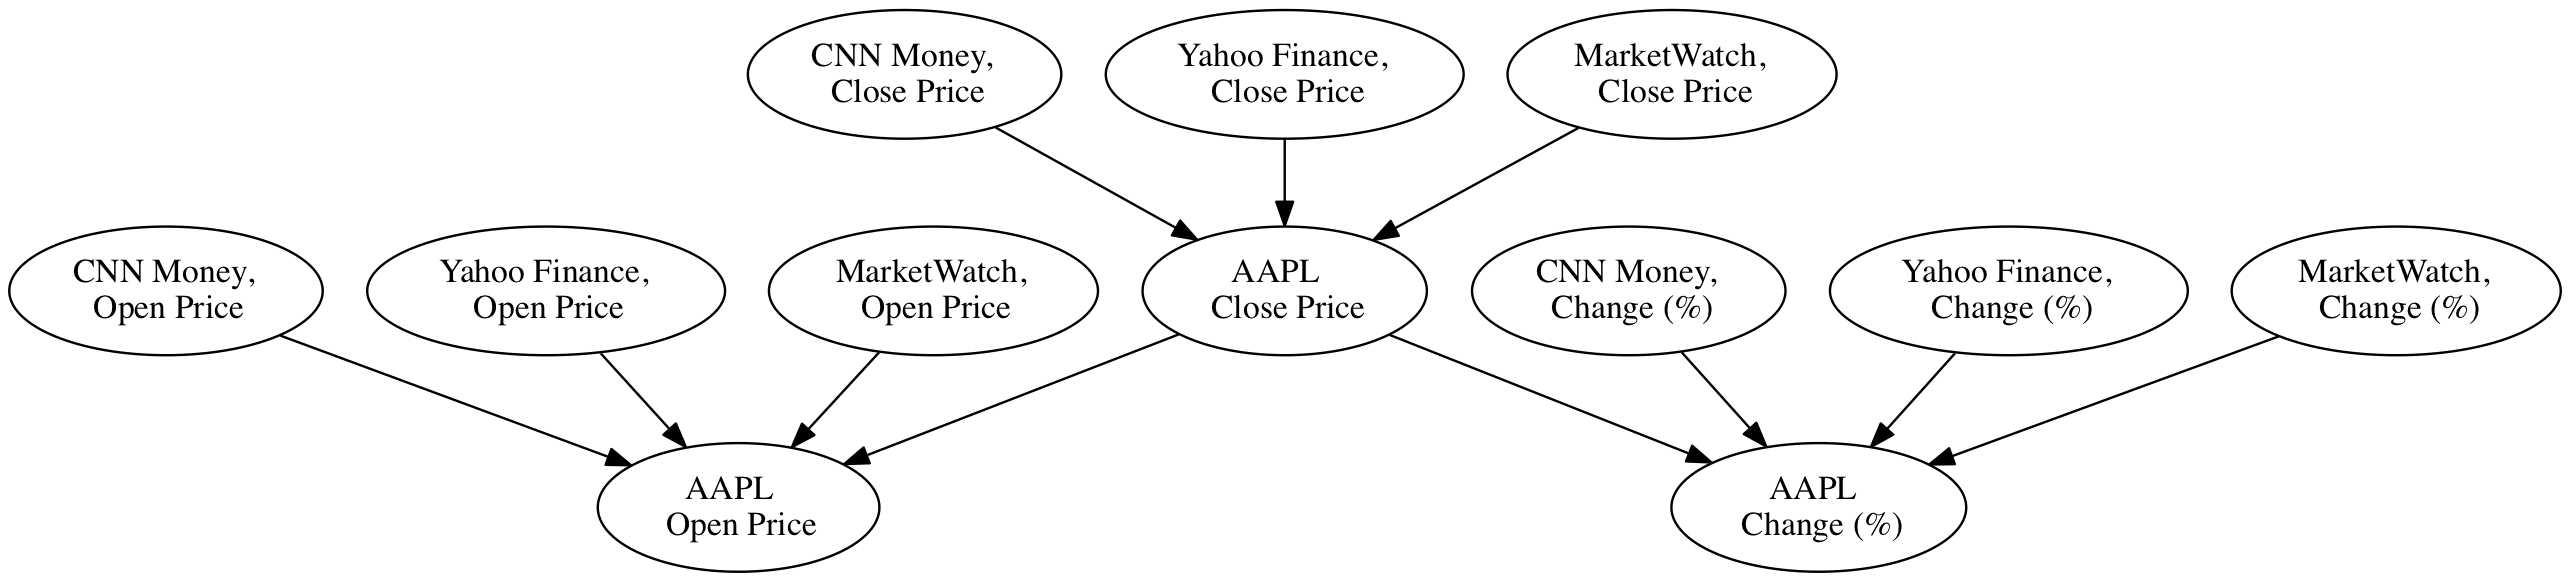
\includegraphics[width=9cm]{bn2.png}
\caption{An example of the attribute dependence model which models the trustworthiness of each attribute provided by a source}
\end{figure}

\begin{algorithm}[H]
\caption{Example Algorithm}
\begin{algorithmic}[1]
\Function{ExampleAlg}{$G_1$, $G_2$, $f$} \\
\Comment{Inputs: Two graphs $G_1 = (V_1,E_1)$ and $G_2=(V_2,E_2)$ and a function $f: V_1 \rightarrow V_2$.} \\
\Comment{Output: Returns ...} \\


\For{\textbf{each} $v_1$ \textbf{in} $V_1$}
\If{$f(v_1) \not \in V_2$}
\State \textbf{return} false
\EndIf
\EndFor
\\

\State \textbf{return} true
\EndFunction
\end{algorithmic}
\end{algorithm}  


\bibliographystyle{abbrv}
\bibliography{references}  

\balancecolumns
\end{document}
